\documentclass{beamer}

\usepackage[spanish]{babel}
\usepackage[utf8x]{inputenc}
\usepackage{beamerthemesplit}

\title{Selección de Servicios Web de Máxima Utilidad Con Circuitos}
\author{Daniel Izquierdo}
\date{14 de diciembre de 2009}

\begin{document}

\frame{\titlepage}

%%%%%%%%%%%%%%%%%%%%%%%%%%%%%%%%%%%%%%%%%%%%%%%%%%%%%%%%%%%%%%%%%%%%%%%%%%%%%%%%

\section[Contenido]{}
\frame{\tableofcontents}

%%%%%%%%%%%%%%%%%%%%%%%%%%%%%%%%%%%%%%%%%%%%%%%%%%%%%%%%%%%%%%%%%%%%%%%%%%%%%%%%

\frame
{
\section{Motivación}

\begin{itemize}
\item Explosión en número de servicios y fuentes de datos disponibles
\item Heterogeneidad de servicios concretos y fuentes
\item Diferencias en calidad de servicio existentes en el mundo real
    \item Necesidad de realizar consultas o \emph{workflows} bajo estas condiciones
\end{itemize}
}

%%%%%%%%%%%%%%%%%%%%%%%%%%%%%%%%%%%%%%%%%%%%%%%%%%%%%%%%%%%%%%%%%%%%%%%%%%%%%%%%

\frame
{
\section{Objetivo}
Desarrollar un sistema eficiente y escalable que pueda resolver problemas de
reescritura de consultas o composición de servicios con constantes, tomando en
cuenta parámetros de calidad para obtener una mejor solución.
}

%%%%%%%%%%%%%%%%%%%%%%%%%%%%%%%%%%%%%%%%%%%%%%%%%%%%%%%%%%%%%%%%%%%%%%%%%%%%%%%%

\frame
{
\section{Retos}
\begin{itemize}
\item Gran número de fuentes o servicios.
\item Manejo de transitividad en asociaciones de variables con constantes.
\end{itemize}
}

%%%%%%%%%%%%%%%%%%%%%%%%%%%%%%%%%%%%%%%%%%%%%%%%%%%%%%%%%%%%%%%%%%%%%%%%%%%%%%%%

\frame
{
\section{Solución Propuesta}
\begin{enumerate}
\item Traducir instancias del problema a instancias de SAT (ya realizado).
\item Añadir cláusulas para tratar con constantes.
\item Compilar teorías a d-DNNF.
\item Calcular todas las reescrituras -- o la mejor.
\end{enumerate}
}

%%%%%%%%%%%%%%%%%%%%%%%%%%%%%%%%%%%%%%%%%%%%%%%%%%%%%%%%%%%%%%%%%%%%%%%%%%%%%%%%

\section{Resultados Estudio Experimental}

\subsection{Vuelos con escalas y aerolíneas}
\frame
{

\begin{center}
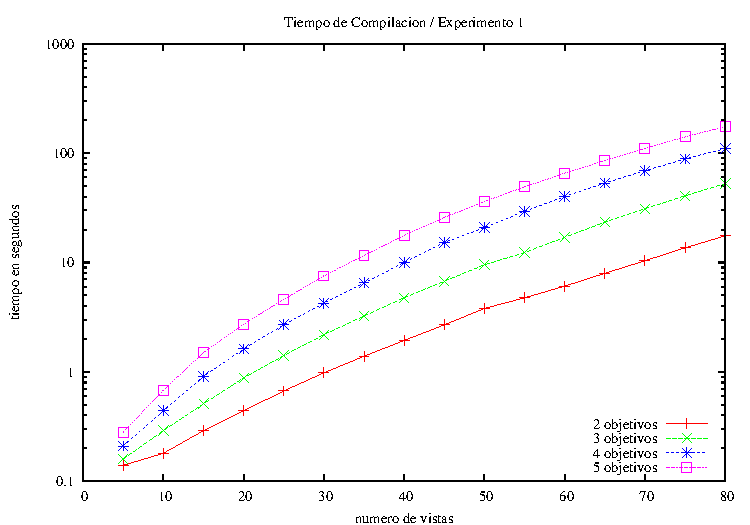
\includegraphics[width=0.5\textwidth]{plot1}
\end{center}

\begin{itemize}
\item Instancias de tamaños realistas
\item Buenos tiempos incluso para las instancias más grandes
\end{itemize}

Esto incluye cálculo de todas las reescrituras o de la mejor.
}

\subsection{Otros experimentos}
\frame
{
\begin{itemize}
\item Con dos vistas por aerolínea: compilación un minuto en caso más grande
\item Menos de seis minutos para problema aleatorio con
\begin{itemize}
\item 80 vistas
\item 5 objetivos de consulta
\item 4 predicados por vista
\end{itemize}

\end{itemize}

Tiempos dados para cálculo de todas las reescrituras.
}

%%%%%%%%%%%%%%%%%%%%%%%%%%%%%%%%%%%%%%%%%%%%%%%%%%%%%%%%%%%%%%%%%%%%%%%%%%%%%%%%

\section{Conclusiones y Trabajo Futuro}

\frame
{
\begin{itemize}
\item Se puede escalar a tamaños razonables.
\item Es factible manejar constantes y rendimiento con la aproximación
propuesta.
\item Se podría pensar en aun más escalabilidad: posible combinación de este
sistema con algoritmo tipo branch and bound.
\end{itemize}
}

\end{document}
